\section{Эксперемент}
\begin{figure}[h]
    \centering
    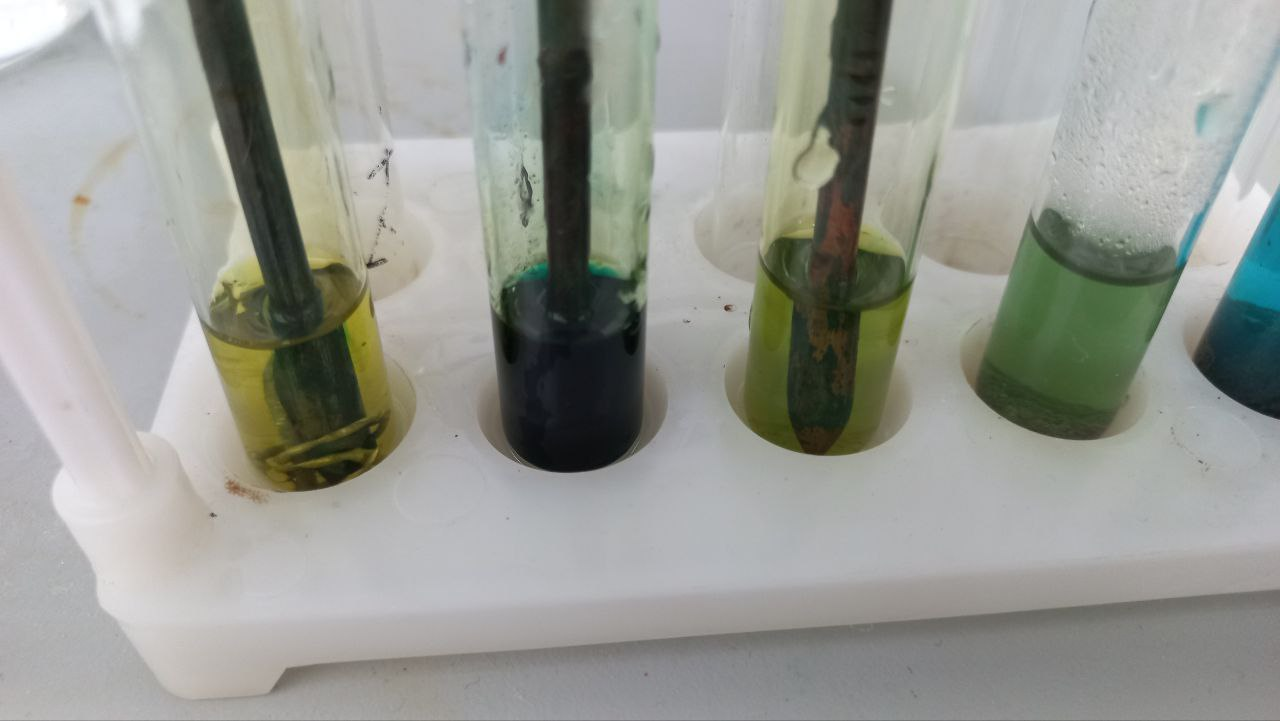
\includegraphics[width=1\linewidth]{Ex_3/Ex_3_1.jpg}
     \caption{Результыты эксперемента}
    \label{Ex_3_1}
\end{figure}

Смотря наблюдая за рекцией можно судить, что: 

\tab 1. В Пробирке с добавлением цинка ракци я окисления практически не идет.

\tab 2. В пробирке с медью рекция идеть активнее всего.

Такое поведение возможно можно былоло бы объяснить 
тем что цинк как более актиыный принемат на себя отрицательно заряженные $OH$
а в случае с медью ситуция обратная. Медь с железом образуют полноценный 
гальвонический элемент где в качестве катода выступат железо, и теперю 
оно выступакт в качестве востановителя.



